\documentclass[10pt]{article}
\usepackage[utf8]{inputenc}\usepackage[T1]{fontenc}\usepackage[letterpaper,margin=1.55cm]{geometry}
\usepackage{graphicx,booktabs,xcolor,amsmath,hyperref,array}\definecolor{navy}{HTML}{102A43}\definecolor{teal}{HTML}{2A9D8F}
\hypersetup{colorlinks=true,urlcolor=teal}\setlength{\parindent}{0pt}\setlength{\parskip}{5pt}
\begin{document}\begin{titlepage}\pagecolor{navy}\color{white}\raggedright\vspace*{1cm}{\Large DEEP LEARNING Y SISTEMAS INTELIGENTES\par}\vspace{1cm}{\Huge\bfseries Proyecto 1\\Monitoreo transaccional --- V3\par}\vspace{.7cm}{\LARGE LightGBM nativo, recencia y validación temporal\par}\vfill{\Large Universidad del Valle de Guatemala\\Kevin Recinos · Grupo 1 · Sección 30\\Semestre II 2026\par}\vspace{1cm}{\Large Wilson Alejandro Calderón Argueta · 22018\\Pablo Daniel Barillas Moreno · 22193\par}\vfill\textbf{Estado:} V3 promovida por cuatro criterios. Benchmark final histórico reutilizado.\end{titlepage}\nopagecolor

\section*{Resumen ejecutivo} Se analizaron 590,540 transacciones IEEE-CIS con prevalencia 3.50%. V3 amplía a 220 variables numéricas y 24 categóricas, conserva ausencias, declara categorías nativas y pondera recencia. Ganó tres de tres ventanas y elevó AP walk-forward de 0.4727 a 0.5809. En el holdout de umbral redujo costo 18.8\% y aumentó recall. Se promueve V3; la confirmación requiere una cohorte nueva.

\section{Datos, identidad y fuga} Las tablas se unen con TransactionID y ordenan con TransactionDT; ninguna entra como magnitud predictiva. Para cada $t$, $x_t^{hist}=f(\{x_j:t_j<t\})$. Se crean conteos previos, media/desviación de monto, razón de monto, tiempo desde operación anterior y actividad 1/6/24/72 h. La clave de tarjeta--dirección genera 42,946 proxies; puede mezclar o fragmentar usuarios. El protocolo usa 70\% train, 15\% validación y 15\% benchmark reutilizado.

\section{Selección y modelos} Correlación e información mutua se aprenden en el 55\% inicial. Se excluyen IDs, constantes y ausencia extrema; la poda $|\rho_s|\ge0.995$ solo elimina sustitutos casi monotónicos. LightGBM usa categorías nativas y NaN; se comparan pesos uniformes, vida media de 75 días y 300k recientes. Como control se ajustan logísticas L2, L1, Elastic Net y PCA64. Las tres variantes SAGA no convergieron en 100 iteraciones y se tratan como baselines diagnósticos.

\begin{figure}[h]\centering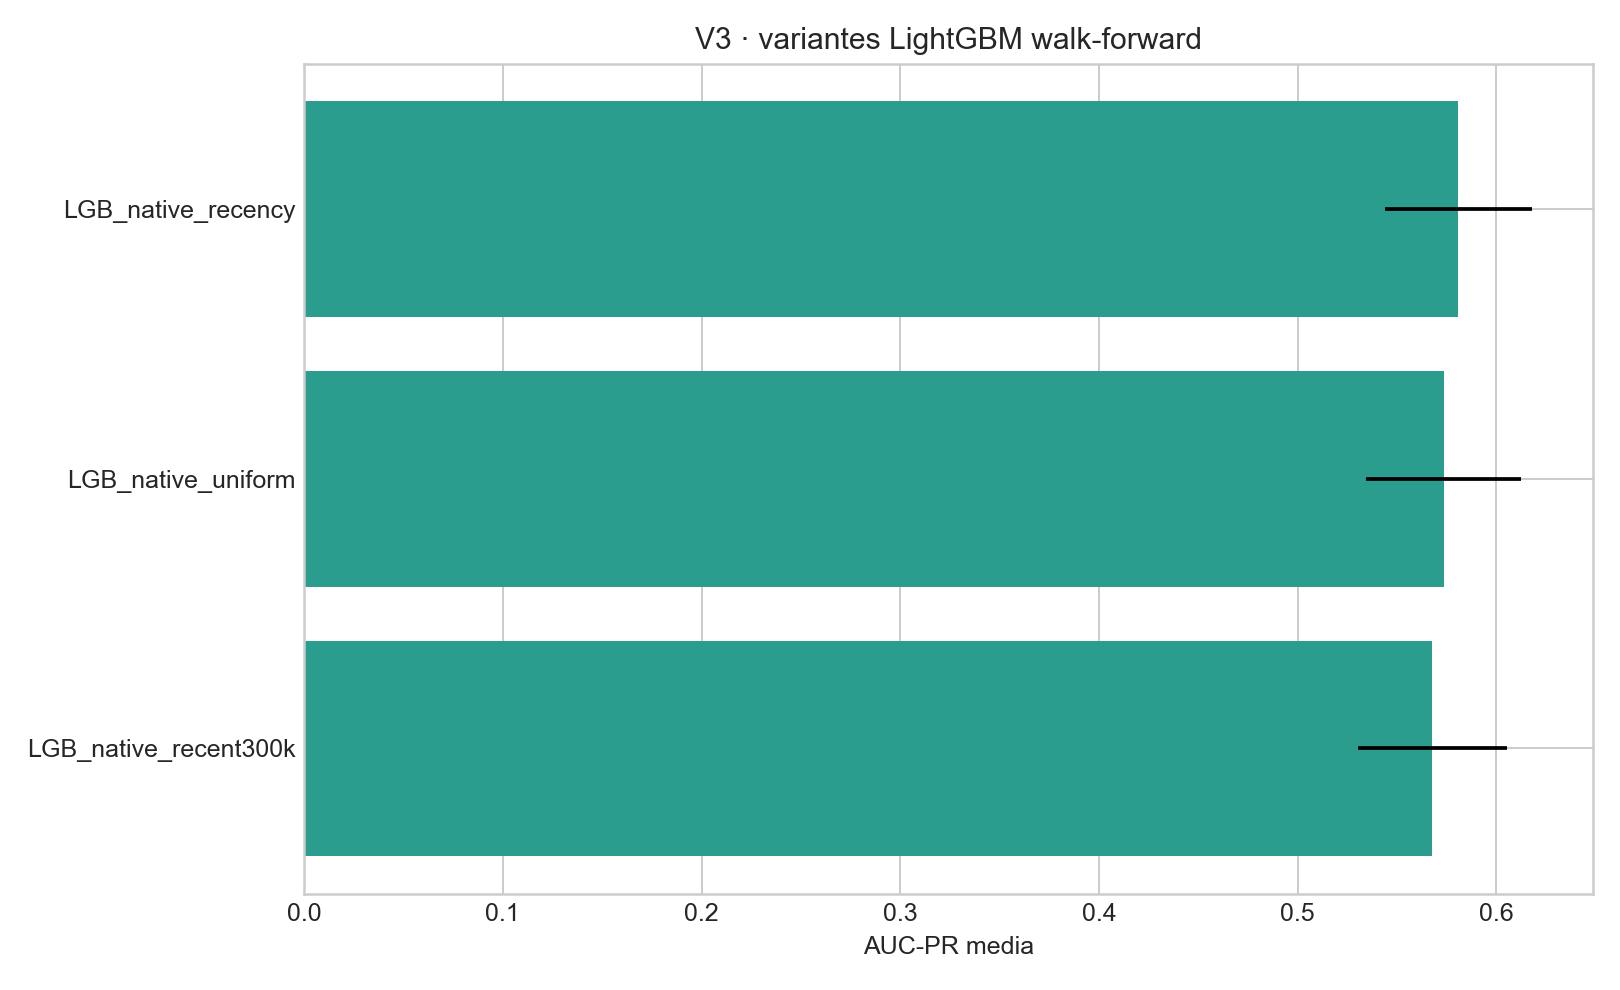
\includegraphics[width=.78\linewidth]{../../../evidencia/figuras/v3/01_walk_forward_v3.png}\caption{Comparación walk-forward de V3.}\end{figure}
\newpage
\section{Validación temporal} Las AP medias fueron 0.5809 con recencia, 0.5735 uniforme y 0.5679 con 300k recientes. Recencia gana los tres folds. Frente a V2, el aumento medio es 0.1082; por tanto, supera el mínimo predefinido de 0.015 sin depender de un solo corte.

PCA64 explica 99.53\% de varianza y obtiene AP 0.3032, mientras Elastic Net obtiene 0.3312. Esto confirma que conservar varianza no equivale a conservar señal supervisada y que el problema necesita interacciones no lineales.

\section{Resultados y promoción}\begin{center}\begin{tabular}{lrrrrr}\toprule Versión&AUC-PR&Prec.&Recall&F1&Costo\\\midrule V1&0.429&0.134&0.722&0.226&Q6,193,620\\V2&0.454&0.149&0.703&0.246&Q6,078,120\\\textbf{V3}&\textbf{0.513}&\textbf{0.190}&\textbf{0.727}&\textbf{0.302}&\textbf{Q5,250,540}\\\bottomrule\end{tabular}\end{center}

La promoción no usa el benchmark: exige AP walk-forward +0.015, costo holdout $-3\%$, recall dentro de un punto y ganar al menos dos folds. V3 cumple los cuatro. En el benchmark reutilizado, la diferencia pareada AP es 0.0589, IC descriptivo [0.0431, 0.0748].

\begin{figure}[h]\centering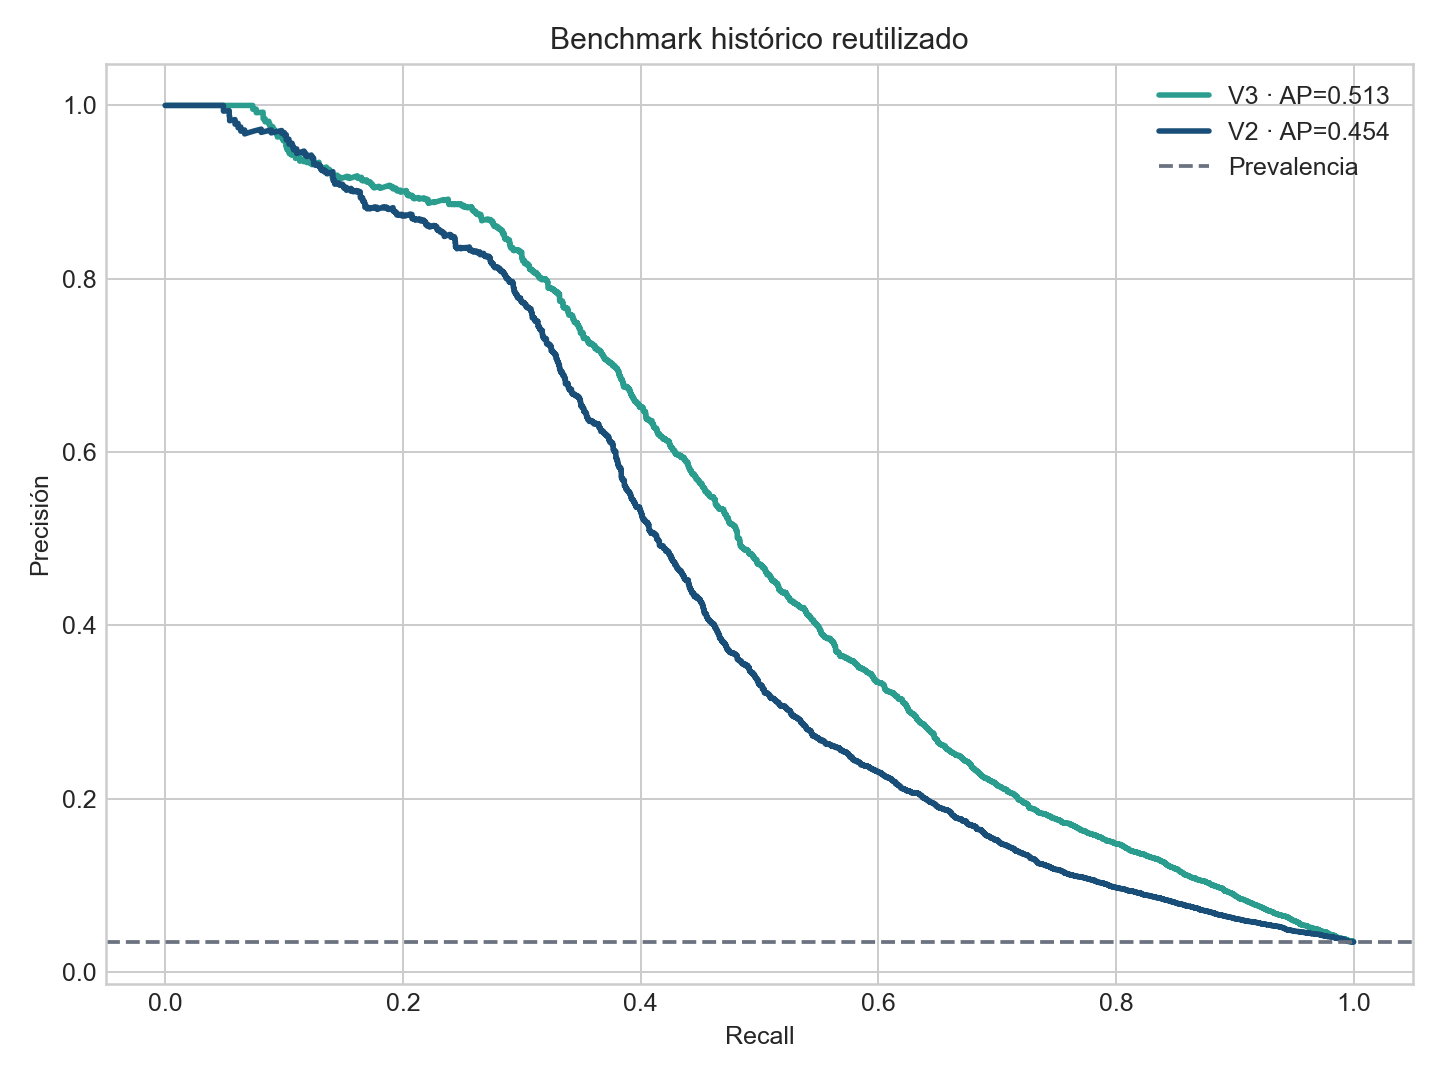
\includegraphics[width=.68\linewidth]{../../../evidencia/figuras/v3/02_curvas_pr_v2_v3.png}\caption{Curvas PR en benchmark histórico reutilizado.}\end{figure}
\newpage
\section{Calibración y umbrales} La validación se divide cronológicamente para early stopping, calibración y selección de umbral. La calibración reduce Brier de 0.0206 a 0.0206 y ECE de 0.0068 a 0.0047.

El umbral balanceado 0.05220 maximiza F1 con recall mínimo 70\%; mejora simultáneamente todas las métricas frente a V2. El umbral económico 0.03164 minimiza $4200FN+180FP$: alcanza recall 0.811 y costo Q5,168,040, pero genera más alertas y menor precisión.

\begin{figure}[h]\centering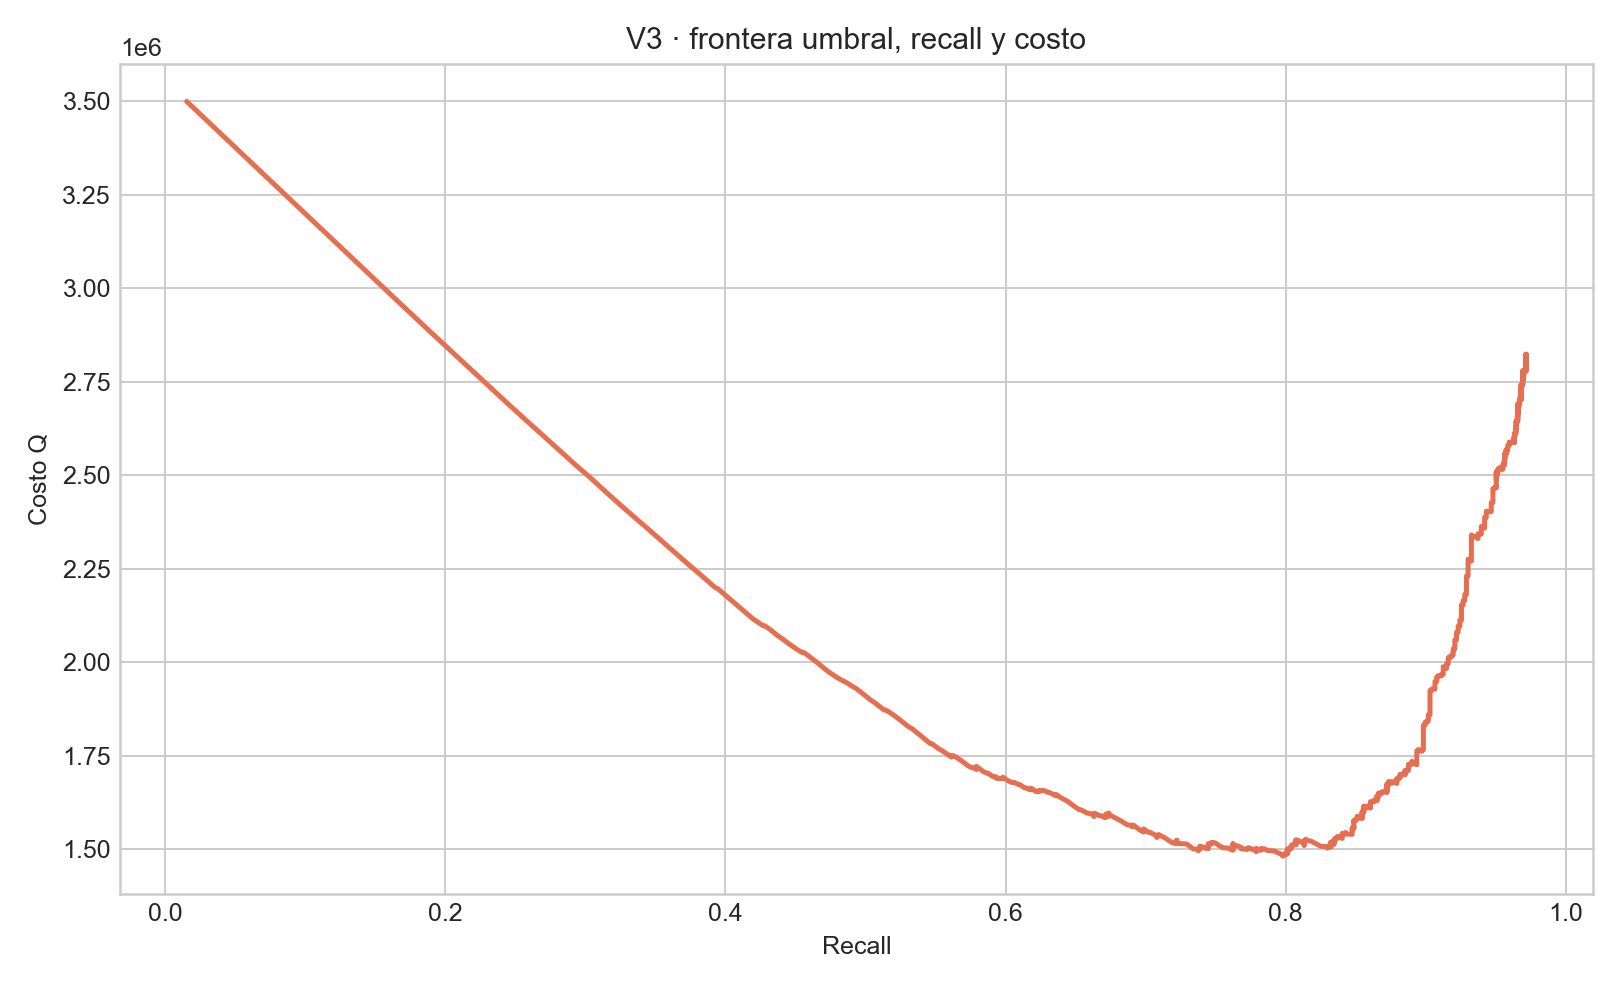
\includegraphics[width=.75\linewidth]{../../../evidencia/figuras/v3/04_costo_recall_v3.png}\caption{Frontera entre recall y costo en el holdout.}\end{figure}

\section{Operación, límites y ética} Al revisar el 1\% de mayor riesgo, precisión es 88.25\% y recall 25.33\%. Se reportan segmentos de producto, dispositivo, monto e historia con el candidato recomendado. El prototipo prioriza revisión humana; no bloquea transacciones ni atribuye culpabilidad.

Limitaciones: benchmark reutilizado, identidad proxy, anonimización, 182 días y costos académicos. Antes de producción se requieren cohorte nueva, privacidad, seguridad, explicabilidad, sesgo, costos reales, latencia y monitoreo de deriva. La GRU no se amplió porque la falsificación V1 no mostró señal de orden suficiente.

\section{Conclusión} V3 mejora de manera significativa y consistente. El salto se atribuye a cobertura ampliada, categorías nativas, ausencia preservada y recencia; regresión logística y PCA no sustituyen las interacciones del árbol. V1/V2 pueden retirarse del árbol activo porque Git conserva su historia y V3 mantiene referencias mínimas para auditoría.

\section*{Referencias}\small IEEE Computational Intelligence Society. (2019). \textit{IEEE-CIS Fraud Detection}. Kaggle.\\Ke, G., et al. (2017). LightGBM. \textit{NeurIPS, 30}.\\Saito, T., \& Rehmsmeier, M. (2015). Precision-recall plots for imbalanced data. \textit{PLOS ONE, 10}(3), e0118432.\\Scikit-learn developers. (2026). \textit{LogisticRegression; Probability calibration}.

\section*{Declaración de IA} IA apoyó código, redacción, visualización y auditoría. Los autores ejecutaron, verificaron y asumen responsabilidad.\end{document}